\documentclass[11pt,letterpaper,notitlepage]{article}

%================== Document nomenclature
\newcommand{\DOCSUBJT}{Whitepaper: }   %Put document subject here
\newcommand{\DOCTITLE}{                      %Put document title here
	Piper Incompressible Liquid - Theory Manual
}       
\newcommand{\DOCDATE} {August, 2023}         %Put document date here
\newcommand{\DOCREV}  {Rev 1.0}             %Put revision number here

%================== Misc Settings
\usepackage{fancyhdr}
\usepackage[left=0.75in, right=0.75in, bottom=1.0in]{geometry}
\usepackage{lastpage}
\usepackage{titleref}
\usepackage{booktabs}
\usepackage{appendix}

\appendixtitleon
\appendixtitletocon

\makeatletter

%================== List of figures and tables mods
\usepackage{tocloft}
\usepackage[labelfont=bf]{caption}

\renewcommand{\cftfigpresnum}{Figure\ }
\renewcommand{\cfttabpresnum}{Table\ }

\newlength{\mylenf}
\settowidth{\mylenf}{\cftfigpresnum}
\setlength{\cftfignumwidth}{\dimexpr\mylenf+3.5em}
\setlength{\cfttabnumwidth}{\dimexpr\mylenf+1.5em}
\renewcommand{\cftsecdotsep}{\cftdotsep} % dotted chapter leaders

\usepackage{bookmark}
\hypersetup{	pdfborder = {0 0 0} }
\setcounter{tocdepth}{5}
\setcounter{secnumdepth}{5}


%=================== Misc packages
\usepackage{graphicx}
\usepackage[breakwords]{truncate}
\usepackage{float}
\usepackage{array}
\usepackage{amsmath}
\usepackage{mdframed}
\usepackage{fancyvrb}
\usepackage{float}
\usepackage{cancel}
\usepackage{amssymb}
\graphicspath{ {images/} }
\usepackage[usenames,dvipsnames,svgnames,table]{xcolor}
%\usepackage[defaultlines=2,all]{nowidow}
\usepackage{listings}
\usepackage{color}
\definecolor{Brown}{cmyk}{0,0.81,1,0.60}
\definecolor{OliveGreen}{cmyk}{0.64,0,0.95,0.40}
\definecolor{CadetBlue}{cmyk}{0.62,0.57,0.23,0}
\usepackage{pdflscape}
\usepackage{relsize}
\usepackage{verbatim}
\usepackage{tabto}
%\usepackage{upgreek}
\usepackage{enumitem}
%\usepackage{MnSymbol}% http://ctan.org/pkg/mnsymbol
\usepackage[pdf]{graphviz}
\usepackage[linesnumbered,lined,boxruled,algosection,commentsnumbered]{algorithm2e}
\usepackage{enumitem}
\usepackage{multicol}
\usepackage{lipsum} %Bunch of garbage paragraphs for testing

\definecolor{gray}{rgb}{0.4,0.4,0.4}
\definecolor{darkblue}{rgb}{0.0,0.0,0.6}
\definecolor{cyan}{rgb}{0.0,0.6,0.6}

\definecolor{ao(english)}{rgb}{0.0, 0.5, 0.0}

\newcommand{\xmltag}[1]{\textcolor{blue}{ \texttt{#1}} }
\newcommand{\xmloption}[1]{\textcolor{ao(english)}{ \texttt{#1}} }


\counterwithin{figure}{section}
\renewcommand{\thefigure}{\arabic{section}.\arabic{figure}}


\newcommand{\beq}{\begin{equation*}
		\begin{aligned}}
		\newcommand{\eeq}{\end{aligned}
\end{equation*}}

\newcommand{\beqn}{\begin{equation}
		\begin{aligned}}
		\newcommand{\eeqn}{\end{aligned}
\end{equation}}

%=================== Settings
\renewcommand{\baselinestretch}{1.2}
\definecolor{gray}{rgb}{0.4 0.4 0.4}
\newcommand{\stimes}{{\times}}

%================== Code syntax highlighting
\lstset{language=C++,frame=ltrb,framesep=2pt,basicstyle=\linespread{0.8} \small,
	keywordstyle=\ttfamily\color{OliveGreen},
	identifierstyle=\ttfamily\color{CadetBlue}\bfseries,
	commentstyle=\color{Brown},
	stringstyle=\ttfamily,
	showstringspaces=true,
	tabsize=2,}

%================== Section numbers with equation numbers
\numberwithin{equation}{section}


%================== Short \to arrow
\setlength{\medmuskip}{0mu}
%\newcommand{\tos}[1][3pt]{\mathrel{%
		%   \hbox{\rule[\dimexpr\fontdimen22\textfont2-.2pt\relax]{#1}{.4pt}}%
		%   \mkern-4mu\hbox{\usefont{U}{lasy}{m}{n}\symbol{41}}}}



%\setlength\parindent{0pt}

%
% Bold quantities
% 
\newcommand{\Omegabf}{\mathbf{\Omega}}
\newcommand{\bnabla}{\boldsymbol{\nabla}}
\newcommand{\position}{\mathbf{x}}
\newcommand{\dotp}{\boldsymbol{\cdot}}

\newcommand{\vel}{\mathbf{u}}
\newcommand{\normal}{\mathbf{n}}
%
% Vector forms
%
\renewcommand{\vec}[1]{\mbox{$\stackrel{\longrightarrow}{#1}$}}
\renewcommand{\div}{\mbox{$\vec{\mathbf{\nabla}} \cdot$}}
\newcommand{\grad}{\mbox{$\vec{\mathbf{\nabla}}$}}
\newcommand{\bb}[1]{\bar{\bar{#1}}}
%
% Vector forms boldfaced
\newcommand{\bvec}[1]{\mathbf{#1}}
\newcommand{\bdiv}{\boldsymbol{\nabla} \boldsymbol{\cdot}}
\newcommand{\bgrad}{\bnabla}
\newcommand{\mat}[1]{\bar{\bar{#1}}}

% Background pic
% Use	\AddToShipoutPicture*{\BackgroundPic} for only current page
% and 	\AddToShipoutPicture{\BackgroundPic} for all pages
%
\usepackage{eso-pic}
\newcommand\BackgroundPic{%
	\put(0,0){%
		\parbox[b][\paperheight]{\paperwidth}{%
			\vfill
			\centering
			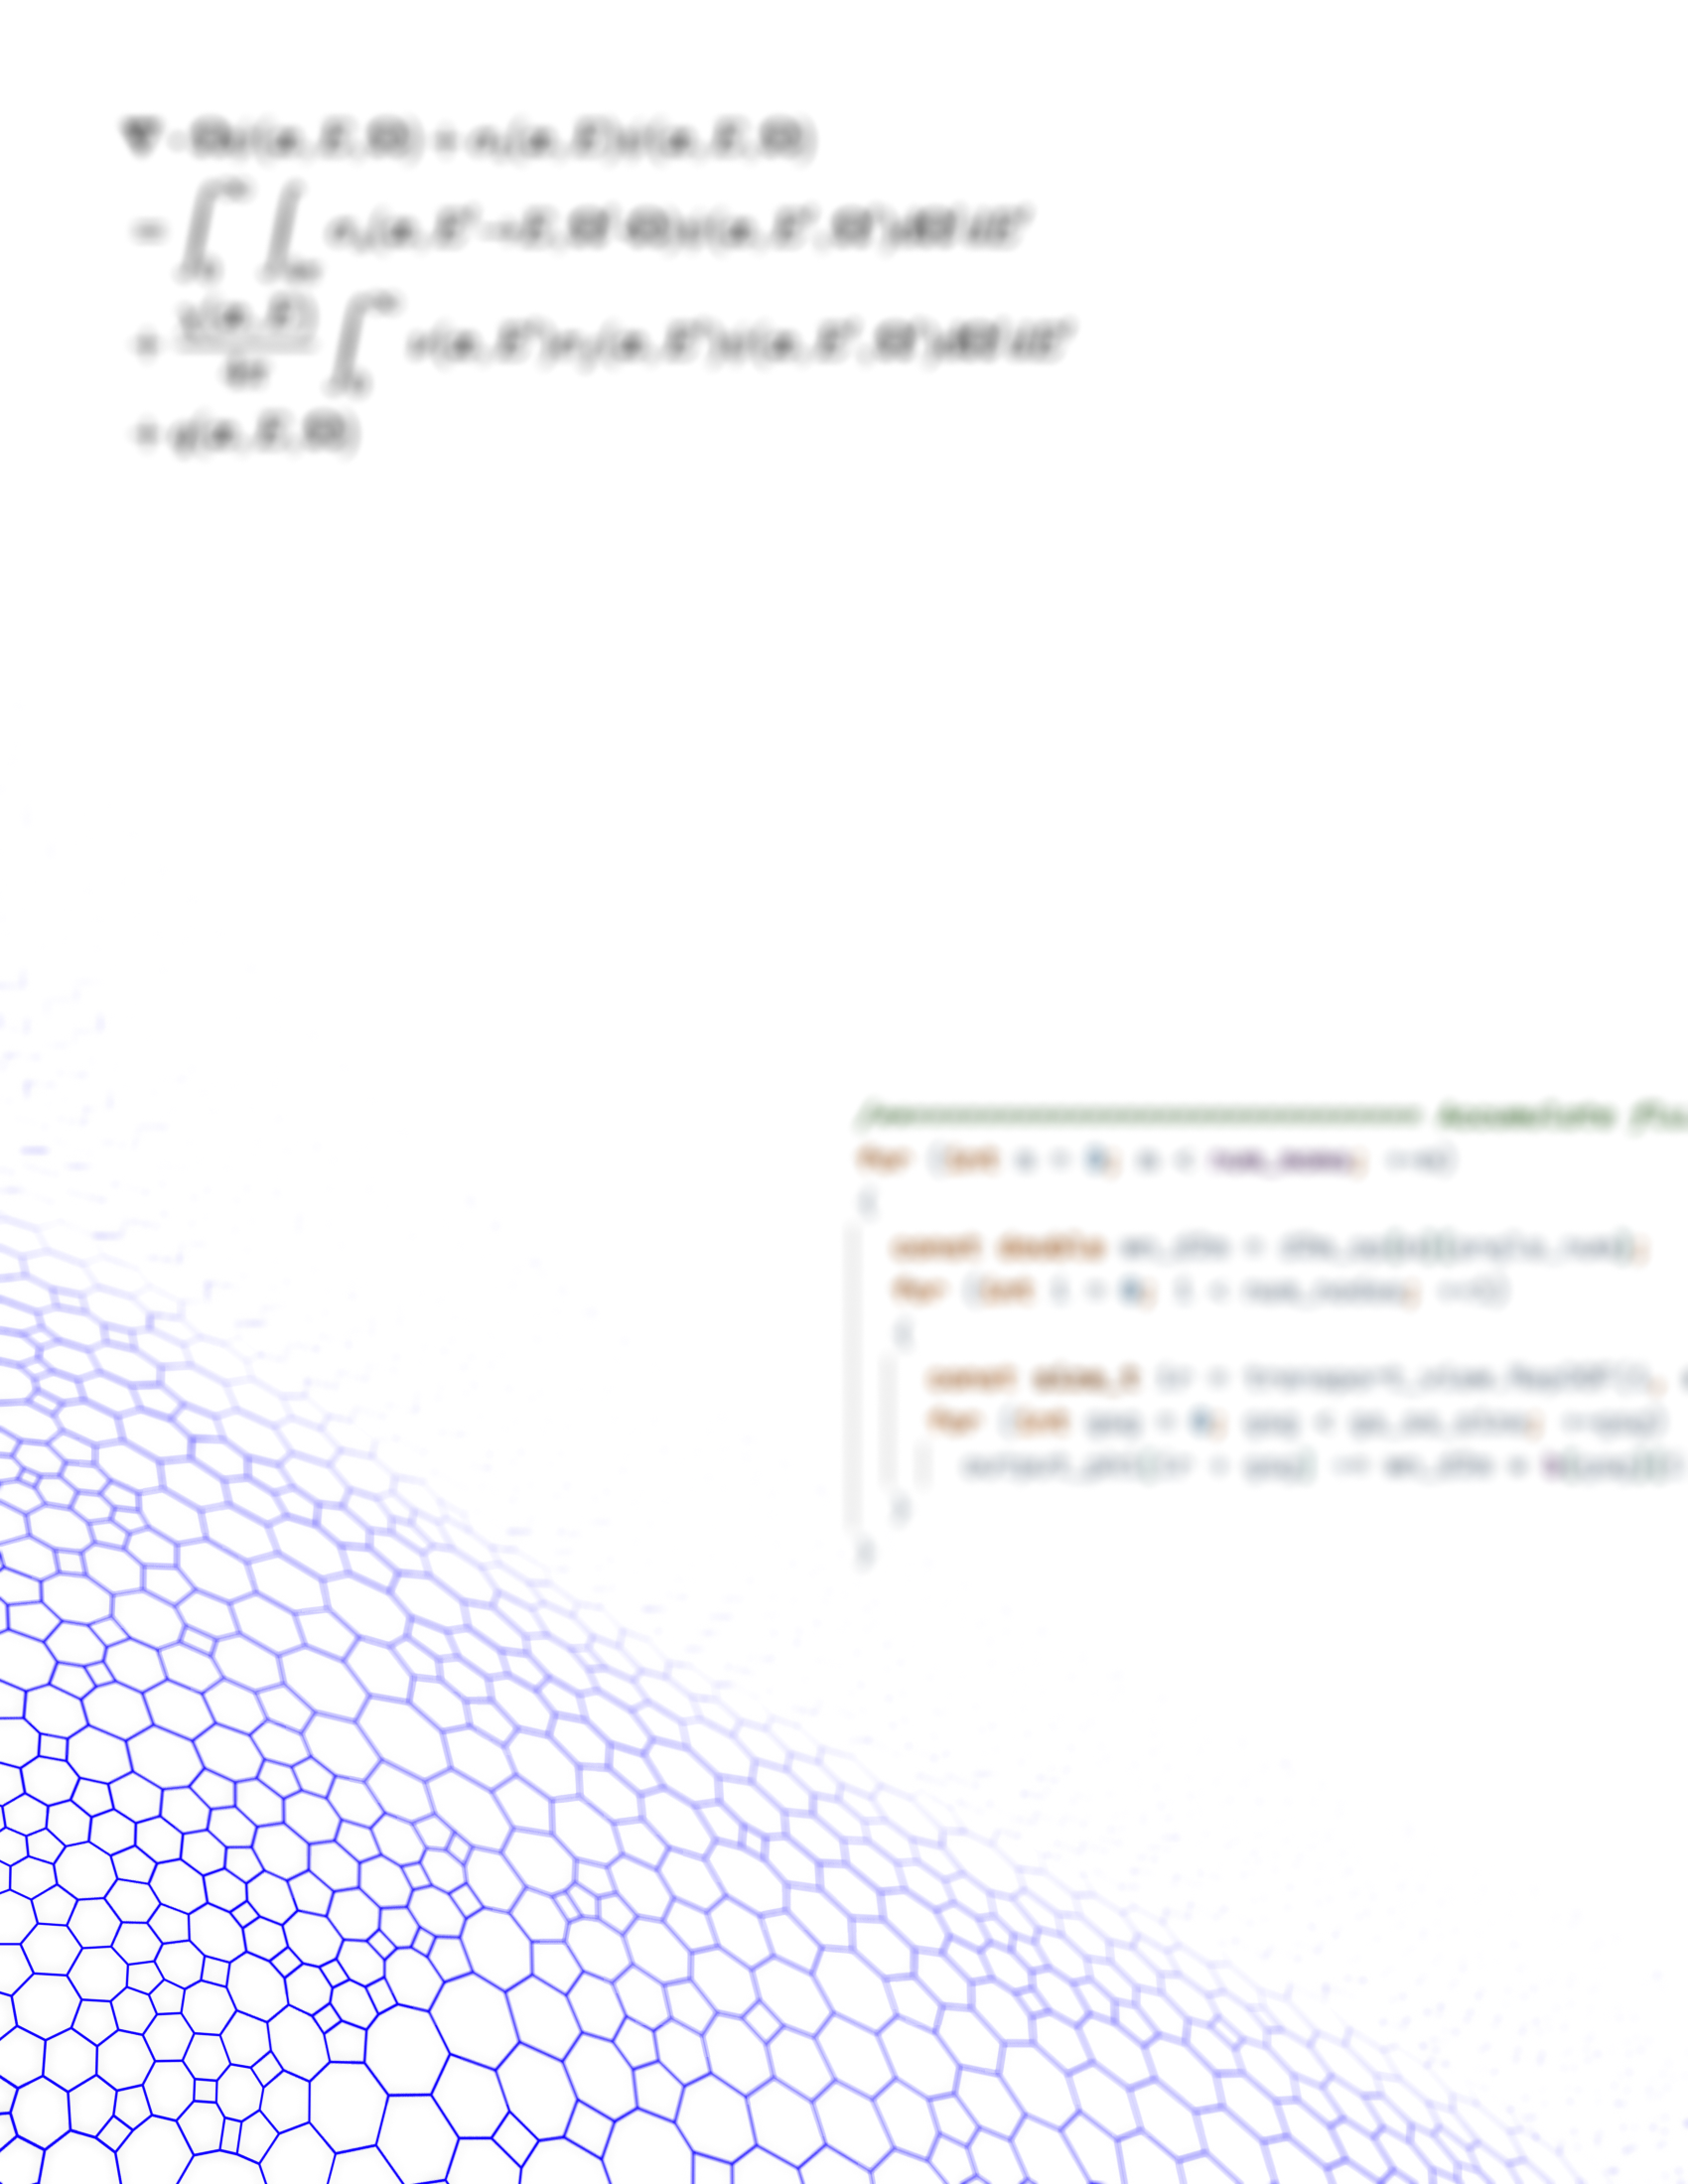
\includegraphics[width=\paperwidth,height=\paperheight,%
			keepaspectratio]{WhitepageBackground.png}%
			\vfill
}}}

%
% Command to make a link back to TOC
%
\newcommand{\BackToTOC}{\hyperlink{toc}{\scriptsize{\color{blue}Back to TOC}}\newline}


\begin{document}
	
\begin{titlepage}
	\AddToShipoutPicture*{\BackgroundPic}
%	\begin{center}
	{\centering 
		\vspace*{3cm}
		{\LARGE\textbf{\DOCSUBJT}}
		
		{\LARGE\textbf{\DOCTITLE}}
		
		\vspace{1cm}
		{\Large \DOCDATE \ \ \DOCREV}
		
		\vspace{1cm}
		{\Large Jan I.C. Vermaak${^{1,2}}$}
		
		\vspace{0.25cm}
		\noindent\rule{\textwidth}{1pt}
		{\small $^1$Idaho National Laboratory, Idaho Falls, Idaho, USA. \\
			$^{2}$ Center for Large Scale Scientific Simulations, Texas A\&M Engineering Experiment Station, College Station, Texas, USA.}
	
%	\end{center}



}
\end{titlepage}

\pagestyle{plain}
%\rfoot{Page \thepage \ of \pageref{LastPage}}
\cfoot{\thepage}
%\lfoot{}
%\rhead{}
%\chead{\currentname}
%\lhead{}
%\renewcommand{\footrulewidth}{0.4pt}
%\setlength{\headheight}{13.59999pt}

\pagenumbering{roman}
\chead{Abstract}
\section*{Abstract}\label{abstract}
\addcontentsline{toc}{section}{\nameref{abstract}}


Work is work for some, but for some it is play.
\newline
\newline\noindent
\textbf{Keywords:} transport sweeps; discrete-ordinate method; radiation transport; massively parallel simulations; discontinuous Galerkin; unstructured mesh

\newpage

\chead{Table of contents}

\tableofcontents
\addtocontents{toc}{~\hfill\textbf{Page}\par \protect\hypertarget{toc}{}}

%
\listoffigures
%%\listoftables





\newpage

\pagestyle{fancy}
\rfoot{Page \thepage \ of \pageref{LastPage}}
\cfoot{}
\lfoot{\truncate{14cm}{\DOCTITLE}}
\rhead{}
\chead{\currentname}
\lhead{}
\renewcommand{\footrulewidth}{0.4pt}
\setlength{\headheight}{13.59999pt}

\pagenumbering{arabic}
%\setcounter{secnumdepth}{1}
\chead{Introduction}
\section{Introduction} \BackToTOC

\chead{Equations}
\section{Equations} \BackToTOC

\subsection{Conservation of Mass}
\beqn 
\frac{\partial \rho}{\partial t} + \bnabla \dotp \rho \vel = 0
\eeqn 

\subsection{Conservation of momentum}
\beqn 
\frac{\partial \rho\vel}{\partial t} + \bnabla \dotp \{ \rho \vel \otimes \vel\} = -\bnabla p + \mathbf{f} + \mathbf{m}_{loss}
\eeqn 

\subsection{Conservation of energy}
\beqn 
\frac{\partial (\frac{1}{2} \rho||\vel||^2 + \rho e)}{\partial t} + 
\bnabla \dotp \biggr[(\frac{1}{2} \rho||\vel||^2 + \rho e + \rho gz)\vel\biggr] +
\bnabla \dotp p\vel = q
\eeqn 

\subsection{Equation of State}
\beqn 
\frac{\partial (\rho e)}{\partial \rho} = F(p, e)
\eeqn 

\newpage
\chead{Numerical schemes}
\section{Numerical schemes} \BackToTOC

\subsection{Semi-implicit time scheme}
With a semi-implicit time scheme we lag certain items in time to gain several advantages. One of the advantages is that we can remove most of the non-linearities.
\newline
\newline
\begin{subequations}
For the conservation of mass equation we lag the density, $\rho$:
	\beqn 
	\frac{\rho^{t+1} - \rho^t}{\Delta t} + \bnabla\dotp \rho^t \vel^{t+1} = 0
	\eeqn 
For the momentum equation we lag the entire momentum in-flux term (containing the velocity tensor), the body force term ($\mathbf{f}$) and the form loss terms ($\mathbf{m}_{loss}$), whilst leaving the pressure gradient implicit:
	\beqn 
	\frac{\rho^t \vel^{t+1} - \rho^t \vel^t}{\Delta t} +
	\bnabla \dotp \{ \rho^t \vel^t \otimes \vel^t \} = -\bnabla p^{t+1} + \mathbf{f}^t + \mathbf{m}^t_{loss}
	\eeqn 
In the energy equation we lag the density, $\rho$, internal energy, $e$, the pressure gradient, $p$, and the heat source, $q$:
	\beqn 
	\frac{(\frac{1}{2} \rho||\vel||^2 + \rho e)^{t+1}-(\frac{1}{2} \rho||\vel||^2 + \rho e)^t}{\Delta t} + 
	\bnabla \dotp \biggr[(\frac{1}{2} \rho^t||\vel^t||^2 + \rho^t e^t + \rho^t gz)\vel^{t+1}\biggr] +
	\bnabla \dotp p^t\vel^{t+1} = q^t
	\eeqn 
Finally, the equation of state we treat explicitly:
	\beqn 
	\frac{(\rho e)^{t+1} - (\rho e)^t}{\rho^{t+1}-\rho^t} = F(p, e)^t
	\eeqn 
\end{subequations}


\newpage
\subsection{Spatial discretization}
For the spatial discretization we employ a finite volume (FV) spatial discretization for all the conservation equations, however, the control volume differs for the different equations as per Figure \ref{fig:controlvolumes} below.
\begin{figure}[H]
	\centering
	\includegraphics[width=0.5\linewidth]{images/ControlVolumes.drawio.pdf}
	\caption{Arrangement of control volumes for the different conservation equations.}
	\label{fig:controlvolumes}
\end{figure}

As a first simplying step we first denote all our conservation equations as 1D:
\begin{subequations}
	\beqn 
	\frac{\rho^{t+1} - \rho^t}{\Delta t} + \partial_x \rho^t u^{t+1} = 0
	\eeqn 
	\beqn 
	\frac{\rho^t u^{t+1} - \rho^t u^t}{\Delta t} +
	\partial_x  \rho^t (u^t)^2  = -\partial_x p^{t+1} + f^t + m^t_{loss}
	\eeqn 
	\beqn 
	\frac{(\frac{1}{2} \rho u^2 + \rho e)^{t+1}-(\frac{1}{2} \rho u^2 + \rho e)^t}{\Delta t} + 
	\partial_x \biggr[(\frac{1}{2} \rho^t (u^{t+1})^2 + \rho^t e^t + \rho^t gz)u^{t+1}\biggr] +
	\partial_x p^t u^{t+1} = q^t
	\eeqn 
\end{subequations}
which simplifies a lot of notation. Next we take the equations one by one and resolve all the terms.
\begin{subequations}
	First is the conservation of mass. This equation is integrated over the volume $i$ and results in
	\beqn 
	V_i\frac{\rho_i^{t+1} - \rho_i^t}{\Delta t} + \sum_j A_{x,j} \rho_j^t u_j^{t+1}  = 0, \\
	\eeqn
	where $\rho_j^t$ is determined using upwinding and the velocity at the junction at the previous timestep, i.e., $u_j^t$.
	
	Next is the momentum equation. Integration here is between the centroids of the adjoining volumes,
	\beqn 
	V_j \frac{\rho_j^t u_j^{t+1} - \rho_j^t u_j^t}{\Delta t} +
	\sum_i A_{x,i} \ \rho_i^t (u_i^t)^2  = -\sum_i A_{x,i} \ p_i^{t+1} + V_j f_j^t + V_j (m_{loss})_j^t,
	\eeqn 
	where $u_i^t$ is taken from the volumetric flow rate average of the adjoing junctions, i.e.,
	\beqn 
	u_i^t = \frac{1}{A_i} \sum_j A_{x,j} u_j^t.
	\eeqn 
	
	Finally, we have the energy equation integral over the volume of control volume $i$,
	\beqn 
	V_i\frac{(\frac{1}{2} \rho u^2 + \rho e)_i^{t+1}-(\frac{1}{2} \rho u^2 + \rho e)_i^t}{\Delta t} + 
	\sum_j A_{x,j} \biggr[(\frac{1}{2} \rho_j^t (u_j^{t+1})^2 + \rho_j^t e_j^t + \rho_j^t gz)u_j^{t+1}\biggr] +
	\sum_j A_{x,j} p_j^t u_j^{t+1} = V_i q_i^t,
	\eeqn 
	where $\rho_j^t$, $e_j^t$ and $p_j^t$ is upwinded using the old velocity.
\end{subequations}


\subsubsection{Neglecting the kinetic energy terms in the energy equation}
When lagging the kinetic energy terms we can obtain a simplification to energy equation.
\beqn 
V_i\frac{(\rho e)_i^{t+1}-(\rho e)_i^t}{\Delta t} + 
\sum_j A_{x,j} \biggr[(\rho_j^t e_j^t + \rho_j^t gz)u_j^{t+1}\biggr] +
\sum_j A_{x,j} p_j^t u_j^{t+1} = V_i q_i^t,
\eeqn 

\subsection{Equations at a glance}
\begin{subequations}
\begin{align}
	a\rho_i^{t+1} + \sum_j a_j u_j^{t+1} &= b 
	\quad \quad \text{ Cons. of Mass}
\end{align}
\begin{align}
	a (\rho e)_i^{t+1} + \sum_j a_j u_j^{t+1} &= b 
	\quad \quad \text{ Cons. of Energy}
\end{align}
\begin{align}
	a u_j^{t+1} + \sum_i a_i p_i^{t+1} &= b 
	\quad \quad \text{ Cons. of Momentum}
\end{align}
\begin{align}
	(\rho e)_i^{t+1} + a_i \rho_i^{t+1} &= b
	\quad \quad \text{ EOS}
\end{align}
\end{subequations}

from which we can see we have the implicit unknowns $\rho_i$, $(\rho e)_i$, $p_i$ and $u_j$.

We now perform some manipulations. Plug EOS into Cons. of Energy
\begin{subequations}
	\begin{align}
		a\rho_i^{t+1} + \sum_j a_j u_j^{t+1} &= b 
		\quad \quad \text{ Cons. of Mass}
	\end{align}
	\begin{align}
		a (\rho )_i^{t+1} + \sum_j a_j u_j^{t+1} &= b 
		\quad \quad \text{ Cons. of Energy2}
	\end{align}
	\begin{align}
		a u_j^{t+1} + \sum_i a_i p_i^{t+1} &= b 
		\quad \quad \text{ Cons. of Momentum}
	\end{align}
\end{subequations}
Now plug Cons. of Mass into Cons. of Energy2.
\begin{subequations}
	\begin{align}
        \sum_j a_j u_j^{t+1} &= b 
		\quad \quad \text{ Cons. of Energy3}
	\end{align}
	\begin{align}
		a u_j^{t+1} + \sum_i a_i p_i^{t+1} &= b 
		\quad \quad \text{ Cons. of Momentum}
	\end{align}
\end{subequations}
Finally, plug Cons. of Momentum into Cons. of Energy3, leaving us an equation with only pressure as the implicit unknown.

\subsection{Detail}
\subsubsection{Cons. of Mass}
\beqn 
V_i\frac{\rho_i^{t+1} - \rho_i^t}{\Delta t} + \sum_j A_{x,j} \rho_j^t u_j^{t+1}  &= 0 
\\
\rho_i^{t+1} - \rho_i^t + \frac{\Delta t}{V_i} \sum_j A_{x,j} \rho_j^t u_j^{t+1} &= 0
\\
\rho_i^{t+1} = - \frac{\Delta t}{V_i} \sum_j A_{x,j} \rho_j^t u_j^{t+1} + \rho_i^t
\eeqn

\subsubsection{Cons. of Energy}
\beqn 
V_i\frac{(\rho e)_i^{t+1}-(\rho e)_i^t}{\Delta t} + 
\sum_j A_{x,j} \biggr[(\rho_j^t e_j^t + \rho_j^t gz)u_j^{t+1}\biggr] +
\sum_j A_{x,j} p_j^t u_j^{t+1} &= V_i q_i^t
\\
(\rho e)_i^{t+1}-(\rho e)_i^t + 
\frac{\Delta t}{V_i} \sum_j A_{x,j} \biggr[(\rho_j^t e_j^t + \rho_j^t gz)u_j^{t+1}\biggr] +
\frac{\Delta t}{V_i}\sum_j A_{x,j} p_j^t u_j^{t+1} &= \Delta t q_i^t
\\
(\rho e)_i^{t+1} + 
\frac{\Delta t}{V_i} \sum_j A_{x,j} \biggr[(\rho_j^t e_j^t + \rho_j^t gz + p_j^t)u_j^{t+1}\biggr] 
&= \Delta t q_i^t+(\rho e)_i^t
\\
(\rho e)_i^{t+1} &=
- \frac{\Delta t}{V_i} \sum_j A_{x,j} \biggr[(\rho_j^t e_j^t + \rho_j^t gz + p_j^t)u_j^{t+1}\biggr] 
\\ &+ \Delta t q_i^t+(\rho e)_i^t
\eeqn 

\subsubsection{EOS}
\beqn 
\frac{(\rho e)^{t+1} - (\rho e)^t}{\rho^{t+1}-\rho^t} &= F(p, e)^t = \frac{\partial (\rho e)}{\partial \rho} \\
(\rho e)^{t+1} - (\rho e)^t &= F(\rho^{t+1}-\rho^t) \\
(\rho e)^{t+1} &= F\rho^{t+1} + (\rho e)^t - F\rho^t
\eeqn 


\subsection{Cons. of Energy2}
EOS:
\beqn 
(\rho e)_i^{t+1} &= F\rho_i^{t+1} + (\rho e)_i^t - F\rho_i^t
\eeqn 
into Cons. of Energy:
\beqn
 (\rho e)_i^{t+1} &=
- \frac{\Delta t}{V_i} \sum_j A_{x,j} \biggr[(\rho_j^t e_j^t + \rho_j^t gz + p_j^t)u_j^{t+1}\biggr] 
+ \Delta t q_i^t+(\rho e)_i^t
\eeqn 
gives:
\beqn
F\rho_i^{t+1} + (\rho e)_i^t - F\rho_i^t &=
- \frac{\Delta t}{V_i} \sum_j A_{x,j} \biggr[(\rho_j^t e_j^t + \rho_j^t gz + p_j^t)u_j^{t+1}\biggr] 
+ \Delta t q_i^t+(\rho e)_i^t 
\\
F\rho_i^{t+1} + (\rho e)_i^t - F\rho_i^t &=
\sum_j a_j u_j^{t+1}
+ b_{COE} 
\\
F\rho_i^{t+1} &=
\sum_j a_j u_j^{t+1}
+ b_{COE} - (\rho e)_i^t + F\rho_i^t
\\
\rho_i^{t+1} &= \frac{1}{F} \sum_j a_j u_j^{t+1} + \frac{1}{F} \biggr(b_{COE} - (\rho e)_i^t + F\rho_i^t\biggr)
\eeqn 

\subsubsection{Cons. of Energy3}
Cons. of Mass:
\beqn
\rho_i^{t+1} &= - \frac{\Delta t}{V_i} \sum_j A_{x,j} \rho_j^t u_j^{t+1} + \rho_i^t
\\
\rho_i^{t+1} &= \sum_j a_j u_j^{t+1} + b_{COM}
\eeqn
into Cons. of Energy2
\beqn 
\rho_i^{t+1} &= \sum_j a_j u_j^{t+1} + b_{COE2}
\eeqn 
Gives:
\beqn 
\sum_j a_j^{COM} u_j^{t+1} + b_{COM} &= \sum_j a_j^{COE2} u_j^{t+1} + b_{COE2} \\
\sum_j (a_j^{COM}-a_j^{COE2}) u_j^{t+1} &= b_{COE2} - b_{COM}
\eeqn 

\subsubsection{What we have thus far}
Cons. of Energy3:
\beqn 
\sum_j a_j^{COE3}u_j^{t+1} &= b_{COE3}
\eeqn
Cons. of Momentum:
\beqn 
V_j \frac{\rho_j^t u_j^{t+1} - \rho_j^t u_j^t}{\Delta t} +
\sum_i A_{x,i} \ \rho_i^t (u_i^t)^2  = -\sum_i A_{x,i} \ p_i^{t+1} + V_j f_j^t + V_j (m_{loss})_j^t,
\eeqn
The latter will be written as
\beqn 
u_j^{t+1} = \sum_i a_i p_i^{t+1} + b_{MOM}
\eeqn 

\subsubsection{Cons. of Mom}
\beqn 
V_j \frac{\rho_j^t u_j^{t+1} - \rho_j^t u_j^t}{\Delta t} +
\sum_i A_{x,i} \ \rho_i^t (u_i^t)^2  &= -\sum_i A_{x,i} \ p_i^{t+1} + V_j f_j^t + V_j (m_{loss})_j^t 
\\
\rho_j^t u_j^{t+1} &= 
- \frac{\Delta t}{V_j}\sum_i A_{x,i} \ \rho_i^t (u_i^t)^2
-\frac{\Delta t}{V_j} \sum_i A_{x,i} \ p_i^{t+1}
+\frac{\Delta t}{V_j}\sum_i V_i f_i^t 
+\frac{\Delta t}{V_j} V_j (m_{loss})_j^t 
+\rho_j^t u_j^t
\\
u_j^{t+1} &= 
- \frac{\Delta t}{V_j \rho_j^t }\sum_i A_{x,i} \ \rho_i^t (u_i^t)^2
-\frac{\Delta t}{V_j \rho_j^t } \sum_i A_{x,i} \ p_i^{t+1}
+\frac{\Delta t}{V_j \rho_j^t }\sum_i V_i f_i^t 
+\frac{\Delta t}{V_j \rho_j^t } V_j (m_{loss})_j^t 
+u_j^t
\eeqn
\beqn
u_j^{t+1} = \sum_i a_i p_i^{t+1} + b_{COM}
\eeqn 

\subsection{Pressure row i}
Cons. of Energy3:
\beqn 
\sum_j a_j^{COE3}u_j^{t+1} &= b_{COE3}
\eeqn
Cons. of Momentum:
\beqn 
u_j^{t+1} = \sum_i a_i p_i^{t+1} + b_{MOM}
\eeqn 
Cons. of Energy3:
\beqn 
\sum_j a_j^{COE3}\biggr( \sum_i a_i p_i^{t+1} + b_{MOM} \biggr) &= b_{COE3}
\\
\sum_j a_j^{COE3}\biggr( \sum_i a_i p_i^{t+1} \biggr) &=
b_{COE3} - \sum_j \biggr( a_j^{COE3} b_{MOM} \biggr)
\eeqn

\newpage
\begin{thebibliography}{1}
	
	\bibitem{LewisMiller} Lewis E.E., Miller W.F., {\em Computational Methods of Neutron Transport}, JohnWiley \& Sons, 1984
	   
\end{thebibliography}

\newpage
\begin{appendices}
\section{First appendix}
Put ``Lazy reader stuff here".
\end{appendices}

\end{document}